\section{Experimental Design and Evaluation Protocol}
\label{sec:design}

This section separates what has been done from what is planned. Four things have been done: the benchmark was downloaded, verified, sampled and re-verified, and its eligible frame was counted; a 50-case seed set was frozen; an operational smoke capture of OpenAlex responses was captured and replayed offline; and the tooling that will run the evaluation was implemented and validated on synthetic data. Everything else is planned: the coverage pilot, the main sample, the independent verification, the main evaluation and its analysis. Fig.~\ref{fig:pipeline} shows the workflow, and the planned stages are drawn with dashed outlines.

\begin{figure*}[t]
\centering
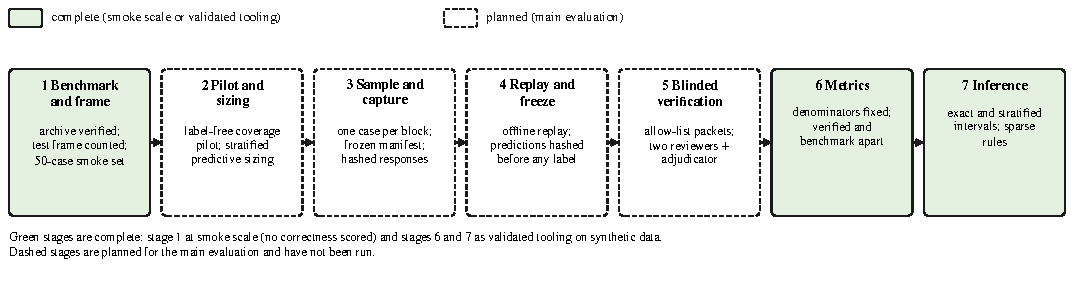
\includegraphics[width=\textwidth]{figures/evaluation_pipeline.pdf}
\caption{Experimental workflow. Completed stages ran at smoke scale only. The label audit, the evaluation and the analysis are planned. Regenerate with \texttt{figures/make\_figures.py}.}
\label{fig:pipeline}
\end{figure*}

\subsection{Benchmark}
\label{sec:benchmark}
The primary benchmark candidate is LAGOS-AND, version 2.0, released on Zenodo (DOI 10.5281/zenodo.7313353) under a CC~BY~4.0 licence~\cite{zhang2022lagosandv2}. The dataset paper and the Zenodo record describe its automatic construction from ORCID and DOI evidence~\cite{zhang2023lagosand}, and the record states that version 2.0 replaces the Microsoft Academic Graph as literature source with OpenAlex. How the ORCID attribution of each individual record was established is not described in the parts of these sources that we could read (the journal version of the dataset paper was not accessible), and we do not assume it.
We used the block-trimmed archive. Its size (743,558,936 bytes) and MD5 checksum matched the values listed by Zenodo, the compressed stream was read to its end, and we computed and recorded a SHA-256 checksum. The archive was processed by streaming. It was obtained a second time and verified again against the same size, MD5 and SHA-256 checksums, and the block catalog built from it reproduced every count in Table~\ref{tab:dataset} and the size-band counts of Section~\ref{sec:seeds}. Table~\ref{tab:dataset} gives the characteristics we measured.

\begin{table}[t]
\caption{LAGOS-AND v2.0 (block-trimmed) as measured by the preparation script.}
\label{tab:dataset}
\centering
\footnotesize
\renewcommand{\arraystretch}{1.1}
\begin{tabular}{@{}p{0.55\columnwidth}p{0.33\columnwidth}@{}}
\toprule
\textbf{Characteristic} & \textbf{Value} \\
\midrule
Data rows & 1,476,550 \\
Name blocks & 80,294 \\
(block, ORCID) identity groups & 244,564 \\
ORCIDs occurring in more than one block & 0 \\
DOIs shared by more than one ORCID & 0 \\
Publication years & 1870 to 2022 \\
Rows without an author affiliation & 14.10\% \\
Blocks eligible for sampling & 70,351 \\
\bottomrule
\end{tabular}
\end{table}

Each block collects publication records for one printed name form, and each identity group within it is defined by an ORCID value attached to its records. A complete pass over all 1,476,550 rows confirmed the publication-year range of Table~\ref{tab:dataset}; an earlier inspection of the first 16,710 rows had shown 1963 to 2022, and the 45 rows dated before 1963 lie outside that prefix. Fourteen columns are present, including the printed author name, affiliation, DOI, publication year, coauthor names and a train, test or validation flag. The \texttt{pid} column behaves like a Microsoft Academic Graph identifier and is not an OpenAlex identifier, and we do not treat it as one. Coauthors are given as name strings without identifiers, so the coauthor-ID signal cannot be observed on this dataset.

The ORCID basis of the groups creates a circularity risk. The expected identity is defined by ORCID equality, and OpenAlex candidate profiles also carry an ORCID field; the two may derive from overlapping upstream attributions. Agreement on ORCID may then reflect shared attribution and not independent verification of the person, and an error in an ORCID attribution could be present on both sides. \textbf{ORCID equality is therefore a provisional matching mechanism and not independent identity ground truth.} The ORCID field also bounds what it can label: in the smoke capture it held a value for only 57.5\% of returned candidates. These are the reasons for the independent verification of Sections~\ref{sec:labels} and~\ref{sec:audit}.

\subsection{Smoke Sample}
\label{sec:seeds}
A deterministic sampler (seed 20261119) built the 50-case smoke sample. The unit of sampling is a complete name block. Blocks with more than eight ORCID groups (2,391) and blocks in which no group has two distinct DOIs (7,552) were excluded. Eligible blocks were stratified by block size alone, using the number of unique DOIs (0--9, 10--49, 50--199 and 200 or more), ordered within each stratum by a hash of the seed and the block name, and taken round-robin only if every query-eligible group of a block fitted the target. No OpenAlex result, ORCID match or HAMMER output was used. The sample has 50 cases from 23 blocks (6, 6, 6 and 5 blocks in the four strata), with 32 train, 15 test and 3 validation cases according to the source flag. HAMMER does not train, so the flag records provenance only. Re-running the sampler on the archive reproduced every output byte for byte, apart from the recorded sampling date.

A seed contains an opaque case identifier, the printed name, an opaque group and block identifier, the context for C1 and for C1x, and sampling metadata. It contains no ORCID, no \texttt{pid} and no coauthor field. The primary C1 context is the affiliation of one designated citation of the group, normalized as described in Section~\ref{sec:affiliation}, and that citation's publication year as a one-year active range. The designated citation is the one with the smallest hash of the seed, ORCID and DOI among those that have an affiliation. Two cases have no affiliation, so their C1 context has no institution. The designated citation is a property of a group member, so it carries a weak hint of group membership. It is the kind of information a user would hold about a new paper, and we record the hint as a design limitation.

The DOI register holds 1,713 DOIs, each used by exactly one case: 1,663 registered as \texttt{gold\_evidence} (the group's other citations) and 50 as \texttt{both} (the designated citation, with a written justification). None is registered as \texttt{query\_context}, so no DOI is present in C1. The 50 designated DOIs form the C1x context. The seeds and the register were hashed and frozen before any candidate was generated.

These 50 cases are an operational pilot sample and are not the main evaluation sample. They are also not 50 independent observations, because the cases come from 23 blocks and cases within a block are related.

\subsection{Smoke Capture}
\label{sec:smoke}
The smoke capture checked whether the toolkit and the provider interface work end to end. It scored no correctness. The capture issued 92 requests, all of which returned HTTP 200: 42 author searches and 50 DOI-based works look-ups for C1x. Fifty cases need 42 and not 50 author searches because R0 and R2 issued identical primary requests in every case and therefore shared one response, ten cases repeat another case's printed name and share its request, and two initials fallbacks were issued. Every response was written to its own file and hashed before the next request. All 92 hashes verified, and the offline replay reproduced its four artifacts byte for byte across two runs. The provider-reported cost was \$0.047. An earlier attempt used a placeholder credential and received 40 HTTP 401 responses. Its records are preserved separately and are not part of the data. The capture now stops at once on HTTP 401, 403 or 429, after saving and hashing the response.

\begin{table}[t]
\caption{Smoke-capture retrieval diagnostics (50 cases, 23 blocks). The expected ORCID is the dataset's, so these counts show label availability and not identity accuracy.}
\label{tab:smoke-retrieval}
\centering
\footnotesize
\renewcommand{\arraystretch}{1.1}
\begin{tabular}{@{}p{0.60\columnwidth}p{0.10\columnwidth}p{0.10\columnwidth}@{}}
\toprule
\textbf{Diagnostic (denominator 50)} & \textbf{R0} & \textbf{R2} \\
\midrule
Expected ORCID found in the pool & 36 & 38 \\
Expected-ORCID profile ranked first & 21 & 22 \\
Expected-ORCID profile within first 5 & 32 & 34 \\
Expected ORCID absent from a successful pool & 7 & 7 \\
ORCID null in every returned candidate & 5 & 5 \\
Successful empty pool & 2 & 0 \\
Provider failure or malformed response & 0 & 0 \\
\bottomrule
\end{tabular}
\end{table}

Table~\ref{tab:smoke-retrieval} lists the retrieval diagnostics. The ORCID field was present on every returned candidate, with a value for 57.5\% of them. The two R0 pools that were empty were found by R2's initials fallback, and the other 48 pools were identical. Rank is the provider's order. These counts describe an ORCID-based diagnostic on one small sample. They do not validate identity retrieval accuracy, and they cannot support a comparison of R0 and R2, because the two shared their primary response in all 50 cases.

\begin{table}[t]
\caption{Smoke-capture replay outcomes (50 cases). No correctness is scored.}
\label{tab:smoke-replay}
\centering
\footnotesize
\renewcommand{\arraystretch}{1.1}
\begin{tabular}{@{}p{0.50\columnwidth}p{0.11\columnwidth}p{0.11\columnwidth}@{}}
\toprule
\textbf{Configuration} & \textbf{Auto} & \textbf{Manual} \\
\midrule
C0, selective\_policy\_v2 & 0 & 50 \\
C1, selective\_policy\_v2 & 4 & 46 \\
C1x (exploratory), selective\_policy\_v2 & 7 & 43 \\
\bottomrule
\end{tabular}
\end{table}

Table~\ref{tab:smoke-replay} lists the replay outcomes under the full policy; every case was either automatic or manual, and none fell into the unresolved, empty-retrieval, provider-failure or no-score categories. The zero in C0 follows from the policy under name-only evidence (Section~\ref{sec:policy}) and is not evidence of safety. C1x remains exploratory: its publication evidence comes from a DOI that is a member of the group, and publication overlap was observed for the top candidate in all 50 cases. Under the threshold-gate ablation with P3 relaxation, C1x yields 26 automatic outcomes, so the safeguard blockers withhold automation in many of the cases that would otherwise pass the threshold gates; whether this improves precision has not been measured. In C1 the institution signal was observed for the top candidate in 29 cases, the candidate had no affiliation in 19 and the query had none in 2, and the temporal signal was observed in 36 and inconclusive in 14. Signal availability, and not only the score, therefore drives the outcome. These counts do not support any claim of precision, recall or superiority over a baseline.

\subsection{Label Strategy and Verification}
\label{sec:labels}
Two kinds of label are kept apart throughout. A \emph{benchmark-derived} label is the provisional ORCID-based mapping of Section~\ref{sec:benchmark}, and it is never described as independently verified. A \emph{verified} label is reached by independent reviewers from evidence outside the benchmark labels (Section~\ref{sec:audit}). A reviewed case has one of four \emph{label states}: resolved (a definite intended person was identified), unresolved (no unique intended person exists), uncertain, or unverifiable. Every case belongs to exactly one \emph{reporting class}: Verified, Uncertain, Unverifiable or Benchmark-derived. Each class is reported with its case count, an audited case is never also Benchmark-derived, and verified and benchmark-derived observations are never combined into one accuracy figure.

The primary population is defined by one condition and policy pair: condition C1 with the full selective policy. Every automatic assignment of that pair is verified independently, and only those assignments define the primary verified precision. A pre-specified random sample of the remaining, non-automatic cases of the same pair is audited. Its frame is the entire non-automatic set, including cases in which no candidate is mapped to the expected person, so that label problems, profile fragmentation and retrieval failure are not excluded. The frame is built after capture and replay under frozen thresholds, weights, code and policy, and it uses no benchmark identity label. The sample is stratified by block size with proportional allocation (largest-remainder rounding) and drawn by a deterministic SHA-256 hash order under a predeclared seed. If strata must be merged, the rule is fixed before the draw and the original stratum sizes are still reported. The audit size is \tbd{set after the reviewer-time pilot}. When a reviewer verifies an automatic assignment, the reviewer receives the complete candidate pool, shuffled and under opaque identifiers, and cannot see HAMMER's selection, rank, score or decision.

Table~\ref{tab:scoring} states how one automatic assignment is scored against its verified label. Only uncertain and unverifiable cases leave the precision denominator. A definite identity without a matching candidate, and a case with no unique intended person, are incorrect assignments and stay in it. Uncertain and unverifiable cases remain visible and are bracketed by counting them all wrong and then all right.

\begin{table}[t]
\caption{Scoring of one automatic assignment against its verified label.}
\label{tab:scoring}
\centering
\footnotesize
\renewcommand{\arraystretch}{1.1}
\begin{tabular}{@{}p{0.50\columnwidth}p{0.20\columnwidth}p{0.13\columnwidth}@{}}
\toprule
\textbf{Verified status; selected candidate} & \textbf{Scored as} & \textbf{In denominator} \\
\midrule
Resolved; judged the same person & correct & yes \\
Resolved; judged a different person & incorrect & yes \\
Resolved; every pool candidate judged different & incorrect & yes \\
Unresolved (no unique intended person) & incorrect & yes \\
Uncertain or unverifiable, or reviewers cannot tell for the selected candidate & not scored, counted & no \\
\bottomrule
\end{tabular}
\end{table}

Benchmark-group validity and case-level candidate verification are separate questions. A reviewer first judges whether the benchmark group is \emph{pure} (all its publications belong to one person), \emph{impure} or \emph{unresolved}. A confirmed impure group is a contradiction of the benchmark label. An uncertain or unverifiable case stays outside the definite-label denominator of the audit error rate even when its group is impure; its impurity is reported separately and the uncertainty bracket is kept. A pure group whose case label is unresolved is indeterminate. For a case with a definite label, the audit error is derived from the adjudicated record and has three reasons: an impure group, a false mapping (a benchmark-mapped candidate judged a different person) and a missed mapping (an unmapped candidate judged the same person). A case counts once in the numerator and the reasons are reported separately. A cannot-tell judgment is indeterminate and never an error.

The audit error rate describes only the sampled non-automatic frame of the primary pair, and it is reported next to the benchmark-derived results of that frame. It is not used as a correction factor, and it is not applied to automatic assignments, to other conditions or policies, or to the overall retrieval results. Conditions and policies other than the primary pair (C0, C1x, the threshold-gate ablation and forced top-one) are reported as benchmark-derived. The benchmark contains only resolved identities, so false acceptance on unresolved queries is not measured, and that measure is omitted.

\subsection{Blinded Review Procedure}
\label{sec:audit}
Review has two stages. In Stage A, reviewers establish who the person is from the printed name and up to $K$ publications of the benchmark group (the designated paper always included, the others chosen and ordered by hash; $K=10$, adopted at the freeze and to be confirmed in the reviewer-time pilot), and they test the purity of the group against evidence outside the benchmark labels. No candidate profile is shown. In Stage B, reviewers judge each candidate of the shuffled pool as the same person, a different person, or undeterminable, against the Stage A identity. Every candidate must be judged before a pool can be declared to hold no matching candidate.

Packets are built by a script from an explicit allow-list of fields and are never edited by hand. The captured provider objects carry the ORCID in several fields (\texttt{orcid}, \texttt{ids.orcid} and an observed-ORCID list), and also identifiers, profile URLs and a relevance score that reveals the provider's rank, so a deny-list would fail silently when the provider adds a field. Stage B packets therefore hold only name variants, affiliation names with years, topics, a works count and yearly counts, and a capped works list from a separate, hashed capture of each candidate's works. Candidates are shuffled by a hash-seeded order that does not depend on the provider's or HAMMER's rank and carry opaque identifiers; the crosswalk to provider identifiers and the flag that says whether a case was automatic or audited are kept in a separate protected location. Automatic and audited cases are presented in the same form and in a mixed queue, so nothing shows a case's origin. Before release a packet is scanned for any ORCID-shaped string, ORCID URL, OpenAlex identifier or URL, rank or score field and HAMMER term, and for any known benchmark value. A packet is released only on zero findings, and its hash is stored with the scan report. Reviewers are asked not to use an ORCID as evidence and to record whether they met one, and results are reported separately for cases in which they did. Residual leakage through a reviewer's own searches cannot be excluded.

Two reviewers judge each case independently. A third person, who is neither a reviewer nor the person who builds the packets, adjudicates disagreements; the final label is recorded with a rationale and never overwrites the reviewers' own rows. Agreement is reported as raw agreement and Cohen's kappa~\cite{cohen1960kappa} together with the counts, because kappa is unstable at small numbers and when one category dominates. Reviewers are outside the project team and have not seen HAMMER outputs or the benchmark ORCID labels for the audited cases; their number, hours and arrangements are \tbd{stated at freeze}. The measured reviewer time of a small pilot on smoke cases sets the audit size.

\subsection{Sampling Design}
\label{sec:sampling}
The main evaluation uses new cases. Its frame is the set of eligible blocks of the test split (Table~\ref{tab:frame}), excluding the 23 smoke blocks and the blocks reserved for the coverage pilot. The study therefore concerns a restricted, benchmark-defined population of ambiguous author blocks (at least two and at most eight ORCID groups); it does not establish performance across all author names or on the most ambiguous names that the cap excludes. Blocks are stratified by the fixed size bands of Section~\ref{sec:seeds}.

\begin{table}[t]
\caption{Eligible blocks of the test split after excluding the 23 smoke blocks, counted from the verified archive. The coverage pilot removes further blocks before the main draw.}
\label{tab:frame}
\centering
\footnotesize
\renewcommand{\arraystretch}{1.1}
\begin{tabular}{@{}lrr@{}}
\toprule
\textbf{Band} & \textbf{Unique DOIs} & \textbf{Eligible blocks} \\
\midrule
S & 0--9 & 8,038 \\
M & 10--49 & 8,360 \\
L & 50--199 & 1,173 \\
XL & 200 or more & 9 \\
\midrule
All & & 17,580 \\
\bottomrule
\end{tabular}
\end{table}

The primary sample takes one case per block: the case-eligible group with the smallest SHA-256 of the seed, block and ORCID. The other case-eligible groups of a drawn block are recorded as secondary cases, are benchmark-derived only, and are used only in an exploratory block-clustered sensitivity analysis. Each ORCID occurs in exactly one block, so one case per block is also one case per person. Within a stratum, blocks are drawn in SHA-256 order of the seed, role and block, which is equivalent to simple random sampling without replacement. Let $N_h$ be the number of eligible blocks in stratum $h$, $n_h$ the number sampled and $g_i$ the number of case-eligible groups in the block of case $i$. A case is included with probability $(n_h/N_h)/g_i$, so the block-level estimand E1 (a random eligible block, then a random eligible person in it) uses the weight $N_h/n_h$, and the person-level estimand E2 uses $(N_h/n_h)\,g_i$~\cite{horvitz1952}. E1 is primary and E2 is secondary, and the two are never conflated.

The allocation across strata is proportional with per-stratum floors. A floor at or above the size of a stratum takes the whole stratum (a census), the remainder is allocated to the unbound strata proportionally to their sizes, and rounding follows the largest-remainder rule. The floors are 0 for strata S, M and L and 9 for stratum XL, which makes XL a census of its nine eligible blocks. Seeds are derived and not chosen: the seed of each role (pilot, main, audit, packet order) is the first eight hexadecimal digits of the SHA-256 of the string \texttt{HAMMER|}\textit{role}\texttt{|}\textit{freeze identifier}, read as an integer, so that no favourable seed can be selected. The total $N$ follows from the pilot (Section~\ref{sec:pilot}). The smoke, pilot and main samples are drawn by separate hash roles and are disjoint. Each draw writes a manifest that holds no ORCID, records the inclusion probabilities as exact fractions and is bound to a SHA-256 of its content and of the selector's source. The mapping from opaque case identifiers to benchmark ORCIDs is held separately.

\subsection{Coverage Pilot and Sample Size}
\label{sec:pilot}
The precision of the verified result depends on the number of automatic assignments, which is random. The share of automatic assignments (coverage) is estimated first by a label-free pilot: a sample of blocks from the test frame, drawn by the same rule with a separate seed and removed from the main frame, is captured and replayed under frozen thresholds, weights, code and policy. The pilot scores no correctness and uses no label, only each case's decision category.

Let $a_h$ be the automatic assignments among $n_{p,h}$ pilot cases of stratum $h$. Coverage $c_h$ is given the prior Beta$(\alpha_0,\beta_0)$, with the Jeffreys prior $(\tfrac12,\tfrac12)$~\cite{jeffreys1946} as the primary choice and the uniform prior as a sensitivity analysis, so $c_h\mid\text{pilot}\sim\text{Beta}(\alpha_0+a_h,\beta_0+n_{p,h}-a_h)$; a stratum without pilot data keeps the prior. For a total sample size $N$, the allocation above gives $n_h(N)$, and the automatic count of stratum $h$ is beta-binomial with parameters $n_h(N)$ and the posterior of $c_h$. The strata are independent, so the distribution of the total $A=\sum_h A_h$ is obtained by exact convolution. The sample size is the smallest $N$ with
\[
\Pr(A\ge m')\ \ge\ 1-\beta
\]
that also holds for every $N'$ up to a declared $N_{\max}$, which guards against non-monotone behaviour of the allocation: largest-remainder rounding can reduce a stratum's share when $N$ grows. The probability $\beta$ is 0.05, the level $\gamma$ is 0.10, $N_{\max}$ is 2,500, and the pilot takes 100, 100 and 50 blocks from the S, M and L strata and none from XL, because all nine XL blocks are needed for the census. Smaller pilots (30 to 40 cases per stratum) left the predictive rule about two percentage points under its target when the prior was mismatched, and $\beta=0.05$ costs about 6 to 7\% more cases than $\beta=0.10$ (Section~\ref{sec:validation}). The target number of automatic assignments $m'$ depends on reviewer capacity, which is not yet known; it is \tbd{fixed after the reviewer-time pilot}, and the main sample size is therefore reported conditionally on $m'$ until then. As a sensitivity check, each $c_h$ is replaced by its exact one-sided Clopper--Pearson lower limit~\cite{clopper1934} at level $1-\gamma/H$ over the $H$ strata (zero without pilot data), and both sample sizes are reported. The rule $N=\lceil m'/c\rceil$ is not used, because it reaches $m'$ only about half the time. The sample size is fixed before the main capture and is not extended after results are seen.

\subsection{Evaluation Metrics}
\label{sec:metrics}
Table~\ref{tab:metrics} defines the measures, their label basis and their denominators. Every drawn primary case stays in the case accounting and falls into exactly one of six outcome categories: automatic, manual, unresolved, successful empty retrieval, provider failure, or no defined score. A case need not be in every denominator. Let $N$ be the number of primary cases. All benchmark labels are resolved, so the \emph{candidate-pool mapping rate} is the share of the $N$ cases whose expected person has a mapped profile in the captured R2 pool; it does not measure the provider's catalog, since a failed search does not show that the person is absent from OpenAlex. R2 is the primary pool for every retrieval measure, and R0 remains a descriptive comparison. \emph{End-to-end} success@$k$ and MRR use all $N$ cases (a failure or an empty pool counts as a miss), whereas \emph{conditional} Recall@$k$ and MRR use only the cases with a mapped profile. The conditional measure alone would let a retriever look effective by excluding the cases in which it retrieved nothing, so the two are always shown together. Overall retrieval is benchmark-derived, keeps all $N$ cases, and is never adjusted by any audit or verified result. Verified retrieval is reported separately, for the automatic assignments and for the audit sample, using only cases with a definite verified label; excluded categories (not yet verified, uncertain, unverifiable, ground-truth unresolved, incomplete judgments) are counted separately, and a HAMMER abstention never removes an otherwise adjudicable case. Its conditional measures use the cases with a verified-same candidate in the pool as denominator, and every other judgment category is reported separately.

\begin{table*}[t]
\caption{Measures, label basis and denominators ($N$ primary cases). Every rate is reported with its numerator and denominator.}
\label{tab:metrics}
\centering
\footnotesize
\renewcommand{\arraystretch}{1.12}
\begin{tabular}{@{}p{0.20\textwidth}p{0.12\textwidth}p{0.34\textwidth}p{0.24\textwidth}@{}}
\toprule
\textbf{Measure} & \textbf{Label basis} & \textbf{Numerator} & \textbf{Denominator} \\
\midrule
Automatic, manual, unresolved, empty, failure and no-score rates & label-free & Cases in the category & All $N$ cases \\
Candidate-pool mapping rate & benchmark & Cases with a mapped profile in the R2 pool & All $N$ cases \\
End-to-end success@$k$, $k\in\{1,5,10\}$; end-to-end MRR & benchmark & Mapped within the first $k$ provider-ordered candidates; reciprocal rank, unmapped counts as 0 & All $N$ cases \\
Conditional Recall@$k$; conditional MRR & benchmark & First mapped profile within $k$; reciprocal rank & Cases with a mapped profile \\
Automatic precision; selective risk & verified & Automatic assignments scored correct (Table~\ref{tab:scoring}); incorrect & Automatic assignments scored correct or incorrect \\
Audit label-error rate & verified & Audited cases with a definite label whose adjudicated record contradicts the benchmark & Audited non-automatic cases with a definite label \\
Verified retrieval, by subset & verified & As for overall retrieval, on verified cases & Cases with a definite verified label, by subset \\
\bottomrule
\end{tabular}
\end{table*}

Precision and coverage are always reported together. When a denominator is zero the measure is reported as undefined and never as zero, and precision is undefined when there are no automatic assignments. The six outcome categories are kept separate in every results table. Retrieval failure, absence of the expected person from the pool and an undecided case are likewise separate. Recall, success and MRR use the provider's order and not HAMMER's score. The coverage and verified precision of other conditions and policies would need their own verification design; they are reported as benchmark-derived.

\subsection{Statistical Inference}
\label{sec:inference}
Strata are finite populations sampled without replacement, so a binomial interval is a model and not the design, and no interval is called design-exact. Three regimes are used. (R1) Per stratum, a Clopper--Pearson interval on the stratum count is reported as a conservative superpopulation approximation; the sampling fraction of each stratum is reported, and a stratum that is a census gets no interval. (R2) The frame-weighted pooled estimate for E1 (and E2) is given with a stratified percentile bootstrap~\cite{efron1979bootstrap} that resamples cases within strata and holds census strata fixed. (R3) Sparse automatic precision is reported as counts with exact intervals, and when there are no errors with the one-sided upper bound $1-0.05^{1/n}$; no bootstrap is used, and a bootstrap on zero errors is never reported. A stratum too small to resample is reported without an interval. The pooled interval is then withheld unless a negligible-weight rule, fixed before the draw, drops that stratum from the pooled estimand, in which case the estimand is relabelled. The numerical warning thresholds (the sampling fraction that flags a stratum, the sparse-count limits, the minimum stratum size for the bootstrap and the contributing-block warning of the clustered analysis) are fixed at the freeze: the sampling fraction that flags a stratum is 0.10, the sparse-count warnings are 30 automatic assignments and 5 errors, the minimum stratum size for the bootstrap is 20 non-census cases, the clustered-analysis warning is 20 contributing blocks, and a stratum with a frame weight below 0.005 is dropped from the pooled estimand and reported separately (this affects only XL, at 0.05\% of the frame). They are diagnostics and not validity boundaries. Paired comparisons between conditions and policies are descriptive and benchmark-derived. A block-clustered bootstrap with a leave-one-block-out check is an exploratory sensitivity analysis on the secondary cases only and is never merged with the primary estimates.

\subsection{Validation of the Evaluation Tooling}
\label{sec:validation}
The evaluation tooling was tested before any evaluation data existed, so that a defect in the tooling cannot be mistaken for a property of HAMMER. The metrics, the sample-size procedure, the selector, the evaluation-freeze manifest, the capture stop-condition guard, the packet builder with its leak scan, the candidate-works capture and release driver, the review-record layer, the report assembly and the table generator were each checked on synthetic data against references that do not share their code: hand-computed values, exact rational arithmetic and independent simulation. In each case, deliberate defects were injected into the code one at a time to confirm that the tests detect them. A synthetic end-to-end rehearsal with a known hidden truth reproduced the verified precision and the audit error rate exactly. On the 50 smoke cases the metrics agreed with an independent diagnostic case by case, and the allow-listed packets built in memory from the 306 captured candidate profiles contained no benchmark ORCID although the raw provider objects did.

Repeated-sampling simulations on a synthetic population were used to check the statistical procedures. The E1 and E2 estimators were unbiased for their own estimands, and applying block-level weights to the person-level target was biased by about twenty standard errors. Per-stratum Clopper--Pearson intervals covered 0.96 to 0.97 at the nominal 0.95. The pooled stratified bootstrap covered 0.935, slightly below nominal. The predictive sample-size rule reached its 0.90 target (0.899) when the true coverage was drawn from its prior, but only 0.88 when the true coverage distribution was narrower than the prior and the pilot was small, whereas the lower-bound check was conservative (0.998) and the rule $N=\lceil m'/c\rceil$ reached 0.55 to 0.68. These are properties of the procedures on synthetic data and not results about HAMMER. They are why per-stratum Clopper--Pearson intervals are reported next to pooled bootstrap intervals, why both sample sizes are reported, and why the size of the pilot matters.

\subsection{Affiliation Cleaning}
\label{sec:affiliation}
Affiliations in the benchmark contain source markers. The seed builder replaces the tab marker \texttt{\#TAB\#} with a space and collapses whitespace, and it keeps the original string in a separate file. Other markers, \texttt{\#R\#\#N\#} and \texttt{\#N\#}, were observed in the sample and are not handled, and some strings contain long multi-institution text. Extending the rule would change the frozen seed and would therefore define a new dataset version. Whether and how to extend it is undecided. The requirements are that the raw affiliation is always preserved, that every transformation is documented, and that the normalizer is separately versioned. No cleaning beyond the tab marker has been done.

\subsection{Status of the Main Evaluation}
\label{sec:main}
The main evaluation has not been run, and no result of it is reported. The protocol above is fixed, and the tooling that executes it has been validated on synthetic data. An evaluation freeze (a manifest of file hashes, the effective configuration, the parameters above and the derived seeds, written before any provider request) and a coverage-pilot draw of 250 blocks have been completed; the pilot leaves 7,938, 8,260, 1,123 and 9 eligible blocks in the S, M, L and XL strata for the main draw. Four freezes (F1 to F4) were written, and the first three were superseded before any usable data existed because the frozen file set had to change: the stop-condition guard was added (F1 to F2), the seed-freeze file written for the capture inputs lacked fields that the capture step verifies (F2 to F3), and the guard mis-handled compressed responses (F3 to F4). The last two defects were found by the first real capture attempts, were fixed with regression tests, and the failed attempts are kept as negative results. The coverage pilot has not been captured and the main sample has not been drawn, because a credential for the provider was not supplied and no money was to be spent. The stop conditions of the capture are: HTTP 401, 403 or 429, an exhausted request budget, three consecutive server errors or transport errors, and 80\% of a cost ceiling. What was captured instead, within the free keyless tier of the provider, is an \emph{exploratory} sample of 50 blocks drawn from the main frame with the derived main seed (disjoint from the smoke and pilot blocks), of which 18 cases were completed before the shared free daily budget ended (Section~\ref{sec:res-samples}). Because that draw consumed the derived main seed, any confirmatory main sample needs a new freeze identifier and must also exclude these blocks. The exploratory results are benchmark-derived and are never used to tune a parameter or to size the confirmatory sample. Still open are the coverage pilot, $m'$ and the resulting $N$, the audit size and merging rule, the confirmatory capture, and the reviewer arrangements, which are not simulated. No setting is tuned on the results of the main evaluation, and a changed protocol is a new version that needs an independent evaluation. The main sample consists of new cases and does not reuse the smoke cases for confirmatory claims. The smoke sample has 50 cases from 23 blocks, which are clustered observations and not 50 independent ones, and no interval is reported for it.
